\chapter{Задание 3. Музыкальное}
\label{ch:chap4}

\definecolor{codegreen}{rgb}{0,0.6,0}
\definecolor{codegray}{rgb}{0.5,0.5,0.5}
\definecolor{codepurple}{rgb}{0.58,0,0.82}
\definecolor{backcolour}{rgb}{0.95,0.95,0.92}

\lstdefinestyle{mystyle}{
    backgroundcolor=\color{backcolour},   
    commentstyle=\color{codegreen},
    keywordstyle=\color{magenta},
    numberstyle=\tiny\color{codegray},
    stringstyle=\color{codepurple},
    basicstyle=\ttfamily\footnotesize,
    breakatwhitespace=false,         
    breaklines=true,                 
    captionpos=b,                    
    keepspaces=true,                 
    numbers=left,                    
    numbersep=5pt,                  
    showspaces=false,                
    showstringspaces=false,
    showtabs=false,                  
    tabsize=2
}

\lstset{style=mystyle}

\section{Построить график ноты}

С этого \href{https://drive.google.com/drive/folders/14lwzvV84uXtyuXXspoYUSf-VdR52t0sE}{гугл-диска} скачиваем два произвольных аккорда,
мой выбор пал на 7-й. Также я перевёл их из mp3 в wav(онлайн конвертер), чтобы можно было их прочитать с помощью SciPy, или можно воспользоваться librosa и открыть сразу.

\begin{figure}[ht]
    \centering
    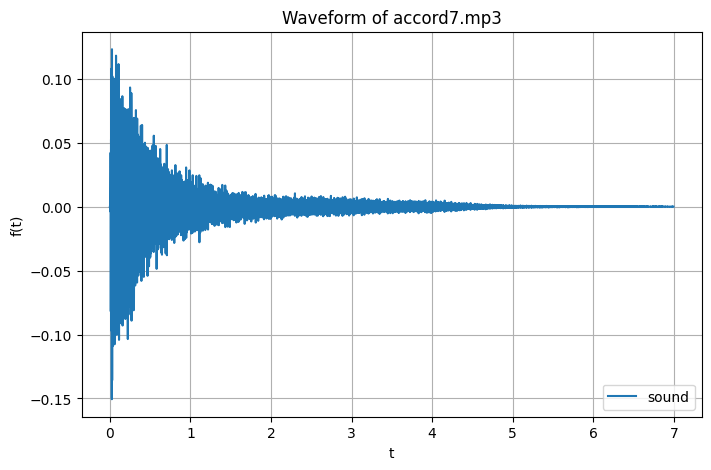
\includegraphics[width=0.8\textwidth]{sound.png}
    \caption{График амплитуды от времени звука}
\end{figure}

\begin{figure}[ht]
    \centering
    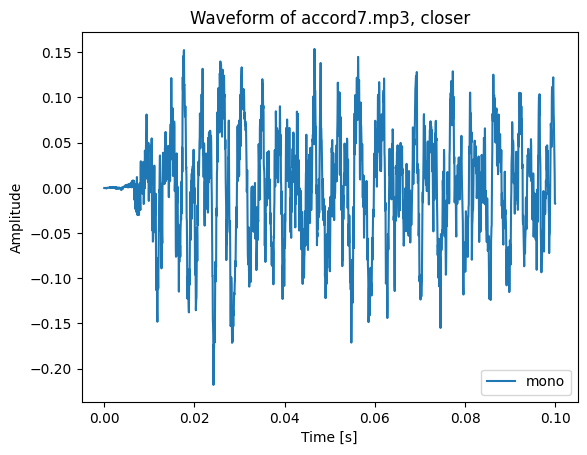
\includegraphics[width=0.8\textwidth]{sound2.png}
    \caption{График амплитуды от времени звука, приблизили}
\end{figure}

\section{Найти численно Фурье-образ}

Из-за того, что интегрирование через Scipy давало странные результаты, пришлось для этого задания ручками написать пару функций, но в итоге удалось всё красиво сделать, модуль образа выглядит корректно, а значит и обычный образ был посчитан правильно.

\begin{figure}[ht]
    \centering
    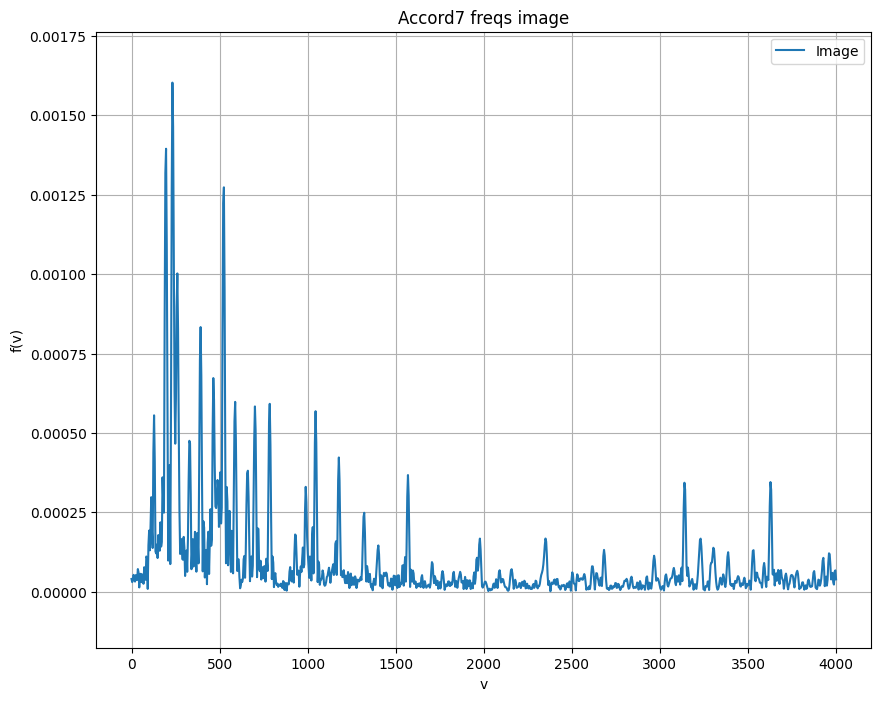
\includegraphics[width=0.9\textwidth]{accord7_freqs.png}
    \caption{Модуль Фурье-образа звука}
\end{figure}


\section{Анализ Фурье-образа}

В моём случае колаб показал, что максимальные амплитуды соответствуют следующим частотам $\in \{232,236,196,192,524,228\}Hz$. Возьмём основные - 524, 236, 196. Найдём одну из многочисленных таблиц в интернете, \href{https://mixbutton.com/mixing-articles/music-note-to-frequency-chart/}{например}, и посмотрим на какие ноты это может быть похоже\dots

Таким частотам соответствуют ноты - C, A\#, G. Интернет мне подсказал, что из таких нот можно составить аккорд Си минор (Cm) или Gm7(септим), первая версия мне знакома больше, поэтому выбираю её.
 







\endinput